
\label{sec:conc}

\subsection{Medición del factor de potencia usando figuras de Lissajou}

Como se discutió en el experimento 1, la medición del $\mathrm{fp}$ se realiza a partir de una relación de amplitudes $A$ y $B$, siendo $A$ la amplitud del canal Y cuando el valor instantáneo del canal X es 0, y $B$ la amplitud de máxima de Y.
Se puede deducir que si existiese un desfasaje de $\phi = 90°$, la amplitud máxima de Y sucedería al mismo tiempo que la mínima de X, y por lo tanto los valores $A$ y $B$ coincidirían $A/B=\sen(90°) = 1$. Por otro lado, la situación extrema opuesta es cuando el desfasaje es de $\phi=0°$, donde se tiene $A=0$, y por lo tanto $A/B = \sen(0°) = 0$.

De esta forma, se puede deducir que la razón de $A$ y $B$ tiene caracter senoidal con respecto $\phi$, y se obtiene la ecuación \ref{eq:Desf} utilizada en la experiencia 1:

\begin{equation*}
    \frac{A}{B} = \sen\phi
\end{equation*}

Entonces el valor del factor de potencia se puede deducir mediante la identidad trigonométrica:

\begin{equation*}
    \begin{aligned}
        \sen^2\phi + \cos^2\phi = 1 \\
        \cos\phi = \sqrt{1-\sen^2\phi}\\
        \cos\phi = \sqrt{1-{\left( \frac{A}{B}\right)}^2}
    \end{aligned}
\end{equation*}



\subsection{Origen de la ecuación de corrección de $\mathrm{fp}$}

La deducción de la fórmula \ref{eq:corrFp} 
de la capacitancia de corrección del factor 
de potencia, se obtiene mediante el análisis
 de la potencia 
Se sabe que para un sistema en atraso con 
una potencia reactiva $Q_L$, la carga capacitiva agregada
debe compensar con una $Q_C$ tal que

\begin{align*}
	Q_C &= Q_L \\
	\frac{V_C^2}{X_C} &= Q_L
\end{align*}

Sustituyendo $Q_L$ por la expresión \ref{eq:visenphi} y bajo
la suposición de que la carga capacitiva se conecta en paralelo con la tensión de alimentación se tiene que:

\begin{equation*}
	 \frac{V^2}{X_C} = V\cdot I \cdot \sen\phi
\end{equation*}

Usando $\sen\phi = \cos\phi\cdot\tan\phi$:

\begin{equation*}
    	\frac{V^2}{X_C} = V\cdot I \cdot \cos\phi\cdot\tan\phi
\end{equation*}
\begin{equation*}
     \frac{V^2}{X_C} = P \cdot\tan\phi
\end{equation*}

\begin{equation}
    C = \frac{P \cdot\tan\phi}{V^2\cdot \omega} 
\end{equation}


\subsection{Generación de armónicas por conmutación capacitiva}

Es conocido que cuando un equipo de compensación de potencia reactiva se instala en redes en las que parte de la carga está constituida por equipos generadores de armónicos, se pueden formar lazos resonantes en varias regiones de la línea. Las corrientes armónicas generadas por los dispositivos no lineales pueden ser peligrosamente amplificadas por la presencia de baterías de condensadores originando valores apreciables de tensiones armónicas superpuestas a la tensión fundamental del sistema, resultando una tensión en barras totalmente distorsionada.

Se debe destacar que los condensadores son cargas lineales, y por lo tanto no crean armónicos por sí mismos, pero si contribuyen a su amplificación.

Al respecto hay que considerar que la impedancia de un condensador se reduce cuando crece la frecuencia, presentando así un camino de baja impedancia para las corrientes de las armónicas superiores. Por su parte, los condensadores de corrección del factor de potencia forman un circuito paralelo con el transformador. Así las corrientes armónicas generadas por los elementos no lineales se dividen entre las dos ramas de este circuito paralelo, dependiendo de la impedancia presentada por el circuito para cada armónico. De esta manera, la corriente eficaz que pasa a través del condensador y por la red de distribución puede aumentar significativamente, y si antes de la corrección había un armónico con una amplitud considerable, entonces la distorsión será más notable debido a la baja impedancia del banco de capacitores en alta frecuencia.

\subsection{Medición de factor de potencia en carga resistiva}
Como ya se explico en la sección \ref{sec:fp}, el factor de potencia es una medida de la eficiencia con la que una carga eléctrica convierte la energía eléctrica en trabajo útil. Para una carga puramente resistiva, el factor de potencia es 1, lo que significa que la corriente está en fase con la tensión. Sin embargo, cuando hay componentes inductivos o capacitivos en la carga, la corriente puede desfasarse con respecto a la tensión, lo que resulta en un factor de potencia menor que 1.

Por lo tanto, en el experimento número 5, es posible que la lámpara utilizada, a pesar de ser predominantemente resistiva, tenga ciertos componentes inductivos o capacitivos que estén causando el factor de potencia menor que 1. Esto consideramos que puede ser atribuible a la presencia de bobinas o condensadores dentro de la lámpara o a la configuración del circuito en el que se encuentra conectada la lámpara.
\subsection{Cotas de corrección}
Las cotas de corrección para señales son un factor que se multiplica el $RMS_{medio}$ de la señal para determinar su valor eficaz real. En los casos de señales sinusoidales, el valor medio de una señal rectificada de amplitud $V_p$ se puede calcular utilizando $V_{media} = \frac{2\cdot V_p}{\pi}$, y además, se sabe que el valor eficaz de esta señal simplemente será $V_{ef} = {V_p\over\sqrt{2}}$. Un multímetro que mide el valor eficaz a partir del valor promediado de la señal, debe multiplicar a $V_{media}$ por un ponderador constante para obtener $V_{ef}$. Este ponderador se puede calcular haciendo:

\begin{equation}
    \begin{aligned}
    V_{ef} &= P \cdot V_{media} \\
    V_p\over\sqrt{2} &= P \cdot \frac{2\cdot V_p}{\pi} \\
    P &= \frac{\pi}{2\cdot\sqrt{2}} \approx 1.11
    \end{aligned}
\end{equation}


Sin embargo, este ponderador solo da el resultado correcto cuando se trata de señales sinusoidales. Cuando la forma de onda es otra (rectangular, triangular, etc), se debe aplicar un factor de corrección $\kappa$ a la medición original del valor eficaz ($V_{RMSmedia}$). Para señales de distintas formas el factor de corrección sera distinto.:

\begin{equation}
    V_{TrueRMS}=\kappa\cdot V_{RMSmedia}
    \label{eq:corrCalcTrueRms}
\end{equation}


 En este parte del trabajo práctico se planteó determinar el factor de corrección para las señales cuadradas y triangulares. Se utilizará una expresión general que relaciona las amplitudes pico de las señales con el factor de corrección $\kappa$, y se hace el despeje:
 
 \begin{equation}
    \begin{aligned}
    V_p \cdot C_{eficaz}&=\kappa \cdot P \cdot V_p\cdot C_{media}\\
     C_{eficaz}&=\kappa \cdot P \cdot C_{media}\\
     \kappa&=\frac{C_{eficaz}}{P \cdot C_{media}}
    \end{aligned}
    \label{eq:factorKappa}
\end{equation}

donde para una señal sinusoidal se tiene que $C_{eficaz} = {1\over\sqrt{2}}$ y $C_{media} = {2\over\pi}$

Recordando la definición del valor eficaz:
\begin{equation}
    V_{rms}=\sqrt{\frac{1}{T}\int_{0}^{T_{a}}v^2dt}
\end{equation}
Se plantearon las siguientes señales genéricas:
\begin{figure}[H]
    \centering
    \begin{minipage}{0.49\textwidth}
        \centering
        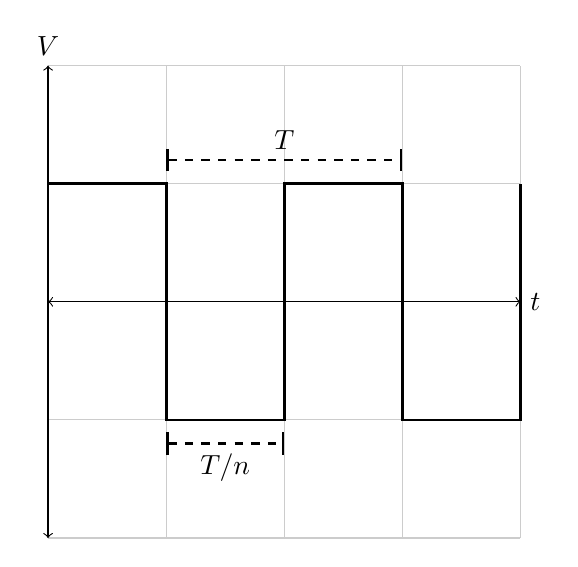
\begin{tikzpicture}[scale=1.5]

    \draw[thin,gray!40] (0,0) grid (4,4);
    
    
    \draw[<->] (0,2)--(4,2) node[right] {$t$};
    \draw[<->] (0,0)--(0,4) node[above]{$V$};

    \draw[line width=1pt,black](0,3)--(1,3)--(1,1)--(2,1)--(2,3)--(3,3)--(3,1)--(4,1)--(4,3);
    \draw[line width=1pt,black,|-|,dashed](1,3.2)--(3,3.2) node[midway,above]{$T$};
    \draw[line width=1pt,black,|-|,dashed](1,0.8)--(2,0.8) node[midway,below]{$T/n$};
\end{tikzpicture}

    \end{minipage}
    \begin{minipage}{0.49\textwidth}
        \centering
        \input{Plots/TriFC}
    \end{minipage}
   
    \caption{Señales de referencia}
    \label{fig:Señref}
\end{figure}

Como se puede observar en la figura\ref{fig:Señref} se asume que la señal cuadrada teniendo en cuenta que el ciclo negativo de la señal es de T/n\%.
Para la señal cuadrada la integral estará dada por:
\begin{equation}
    \begin{aligned}
         V_{rms}=&\sqrt{\frac{2}{T}\int_{0}^{\frac{T}{n}}V_{p}^2dt}\\
         V_{rms}=&\sqrt{\frac{2V_{p}^2\cdot\frac{\cancel{T}}{n}}{\cancel{T}}}\\
         V_{rms}=&\frac{V_{p}\sqrt{2}}{\sqrt{n}}
    \end{aligned}
\end{equation}
Teniendo en cuenta que la señal cuadrada medida en el experimento 3 su ciclo negativo es del 50\%:
\begin{equation}
    V_{rms}=V_{p}
\end{equation}
El factor $C_{eficaz}$ para una señal de este tipo es entonces 1.


Para señales triangulares:
\begin{equation}
    \begin{aligned}
         V_{rms}=&\sqrt{\frac{2}{T}(\int_{0}^{\frac{T}{4}}f_{(t)}^2dt+\int_{\frac{T}{4}}^{\frac{T}{2}}f_{(t)}^2dt)}\\
         V_{rms}=&\sqrt{\frac{2}{T}(\int_{0}^{\frac{T}{4}}(\frac{V_{p}}{T/4}\cdot t)^2)dt+\int_{\frac{T}{4}}^{\frac{T}{2}}((\frac{-V_{p}}{T/4}\cdot t)^2dt)}\\
          V_{rms}=&\sqrt{\frac{64V_{p}^2}{T^3}\int_{0}^{\frac{T}{4}}t^2dt}\\
          V_{rms}=&V_{p}\cdot\sqrt{\frac{64}{3T^3}\cdot(\frac{T}{4})^3}\\
          V_{rms}=&\frac{V_{p}}{\sqrt{3}}\\
    \end{aligned}
\end{equation}
El factor $C_{eficaz}$ para una señal de triangular es entonces $\frac{1}{\sqrt{3}}$.

Ahora el valor medio de estas señales rectificadas sera de:
\begin{equation}
    V_{media}=\frac{\int_{0}^{T} |f_{(t)}|dt}{T}
\end{equation}
\begin{figure}[H]
    \centering
    \begin{minipage}{0.49\textwidth}
        \centering
        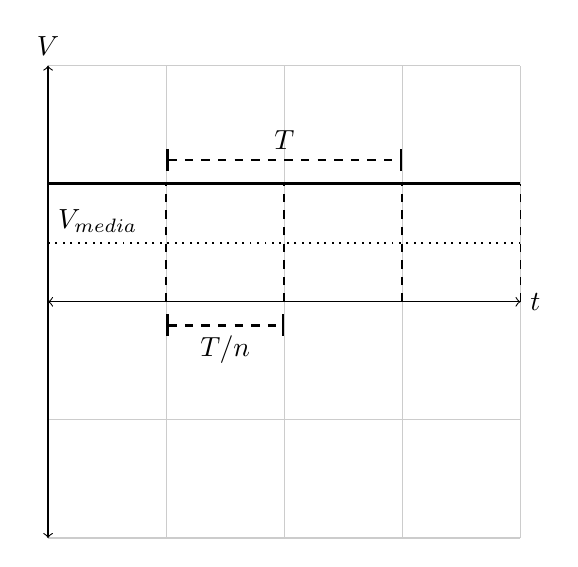
\begin{tikzpicture}[scale=1.5]

    \draw[thin,gray!40] (0,0) grid (4,4);
    
    
    \draw[<->] (0,2)--(4,2) node[right] {$t$};
    \draw[<->] (0,0)--(0,4) node[above]{$V$};
    \draw[line width=0.7pt,dotted](4,2.5)--(0,2.5) node[anchor=south west]{$V_{media}$};
    \draw[line width=1pt,black](0,3)--(4,3);
    \draw[line width=0.7pt,black,dashed](1,2)--(1,3);
    \draw[line width=0.7pt,black,dashed](2,2)--(2,3);
    \draw[line width=0.7pt,black,dashed](3,2)--(3,3);
    \draw[line width=0.7pt,black,dashed](4,2)--(4,3);
    \draw[line width=1pt,black,|-|,dashed](1,3.2)--(3,3.2) node[midway,above]{$T$};
    \draw[line width=1pt,black,|-|,dashed](1,1.8)--(2,1.8) node[midway,below]{$T/n$};
\end{tikzpicture}

    \end{minipage}
    \begin{minipage}{0.49\textwidth}
        \centering
        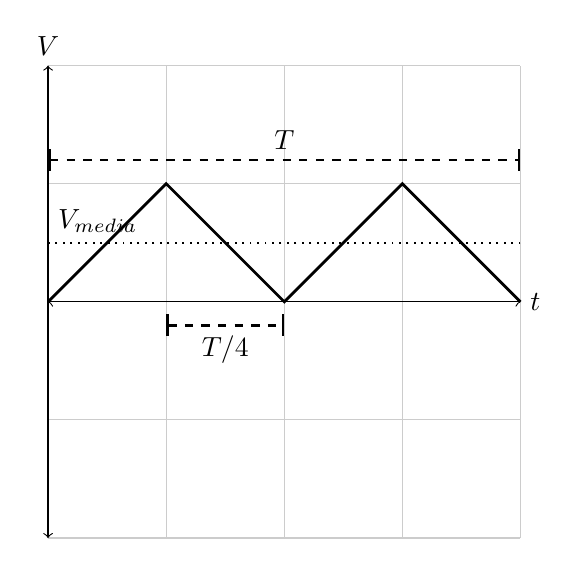
\begin{tikzpicture}[scale=1.5]

    \draw[thin,gray!40] (0,-2) grid (4,2);
    
    
    \draw[<->] (0,0)--(4,0) node[right] {$t$};
    \draw[<->] (0,-2)--(0,2) node[above]{$V$};
    \draw[line width=0.7pt,black,dotted](4,0.5)--(0,0.5) node[anchor=south west]{$V_{media}$};
    \draw[line width=1pt,black](0,0)--(1,1)--(2,0)--(3,1)--(4,0);
    \draw[line width=1pt,black,|-|,dashed](0,1.2)--(4,1.2) node[midway,above]{$T$};
    \draw[line width=1pt,black,|-|,dashed](1,-0.2)--(2,-0.2) node[midway,below]{$T/4$};
    
\end{tikzpicture}

    \end{minipage}
   
    \caption{Señales de referencia}
    \label{fig:Señref}
\end{figure}
Para la señal cuadrada el valor medio es simplemente de:
\begin{equation}
    V_{media}=V_p
\end{equation}
Por lo tanto el factor $C_{media}$ para una señal cuadrada sera de $1$

Y para la señal triangular será de :
\begin{equation}
    \begin{aligned}
         V_{media}=&2\cdot\frac{\int_{0}^{\frac{T}{4}} |f_{(t)}|dt}{T}\\
         V_{media}=&2\cdot\frac{\int_{0}^{\frac{T}{4}} \frac{V_{p}}{T/4}\cdot t dt}{T}\\
         V_{media}=&\frac{8V_{p}}{T^2}t^2|_{0}^{\frac{T}{4}}\\
         V_{media}=&\frac{V_{p}}{2}
    \end{aligned}
\end{equation}
El factor $C_{media}$ será entonces para esta señal $0.5$.

%Ya teniendo todos nuestros factores podemos construir las ecuaciones que el multímetro de valor medio debería utilizar para estas señales:
%\begin{equation}
%    \begin{cases}
%        V_{RMSCuad}=Vp\\
%        V_{RMSTrian}=Vp\cdot0.5772
%    \end{cases}
%\end{equation}
Una vez calculados las constantes $C_{media}$ y $C_{eficaz}$ de la forma cuadrada y rectangular, se procede calcular el factor de corrección $\kappa$ para cada forma. Se utilizará el despeje de la expresión \ref{eq:factorKappa}, dándonos como resultado los siguientes factores de corrección:
\begin{equation}
    \begin{cases}
        \kappa_{Cuad}=\frac{2\sqrt{2}}{\pi} \approx 0.900\\
        \kappa_{Tria}=\frac{4\sqrt{2}}{\pi\sqrt{3}} \approx 1.040
    \end{cases}
\end{equation}

Finalmente, para obtener el valor True RMS, solo debemos multiplicar el valor del multímetro de valor medio ($V_{RMSmedio}$), por el coeficiente que corresponda según la forma de onda (ecuación \ref{eq:corrCalcTrueRms}).

\begin{equation}
    V_{TrueRMS(Cuad)} = \kappa_{Cuad} \cdot V_{RMS(Cuad)}
\end{equation}
\begin{equation}
    V_{TrueRMS(Tria)} = \kappa_{Tria} \cdot V_{RMS(Tria)}
\end{equation}















